\chapter{Method}\label{cha:method}

This thesis report present a algorithm to detect facial marks automatically. This chapter will briefly describe the method used to develop the algorithm. Further details can be found in the referred works. 

\section{Detection}

An overview of the algorithm is presented in figure \ref{fig:detection_flow}. The algorithm consist of several submodules which has it own functionality. Each image, \textit{I}, is processed and go through each of these subsystems. 

\begin{figure}[h]
	\centering
	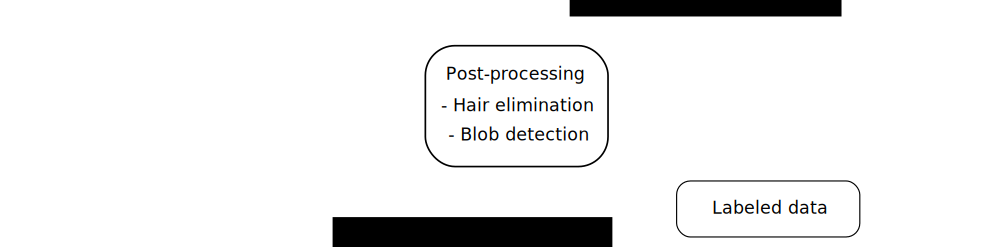
\includegraphics[width=\textwidth,height=\textheight,keepaspectratio]{flow_report}
	\caption{Overview of the algorithm \label{fig:detection_flow}}
\end{figure}

\subsection{Face detection}

An important component for further processing is the bounding box of the face in each image. It is found by using an OpenCV \cite{opencv} implementation of object detection by Paul Viola et al. \cite{face_detection}. This face detection algorithm was chosen since it has equivalent positive result as other methods \cite{face_detecion_comp,face_detecion_comp_2}. In addition, it is much faster the the other detector. The algorithm from Paul Viola et. al. take advantage of three different parts. 

The first is part is a new image representation which allows Haar features from each image to be calculated rapidly. The speed is achieved by using integral images instead of the original image. 

The second part is the extraction of the most important features through AdaBoosting. It creates a strong classifier by combining the strength of weaker classifiers. A weak classifier is the best threshold for a feature which separates the faces from the non-faces.

The third part is a cascade decision which reduces the computations costs by rejecting potential bounding boxes for the face. A simple classifier is used to determine if the bounding boxes are promising candidates before a more complex classifier is engaged. This is repeated until all classifiers has been passed or if one of the returns a negative result. All bounding boxes which has returned a negative result is rejected immediately.  

When a suitable bonding box as been found for \textit{I}, the landmarks in the image can be extracted. 

\subsection{Landmark detection}

To process a facial image, it is useful to know where different parts of the face are located, e.g. mouth and eyes. These parts can be pinpointed with points called landmarks. With these landmarks, it is possible to create a unique mask for each face and produce a grid with different regions in the face. The landmarks are extracted by using an implementation based on Vahid Kazemi et al. \cite{dlib_landmark}. It uses sate of the art algorithms for face alignment where cascade of regression functions are crucial for its success. The estimated shape of the face is updated by regressing the shape parameters based on normalized features from the image. The parameters are updated until they converges.

From this algorithm, 68 landmarks are extracted where the eyes, mouth, nose and chin are marked. From these, a mask generated where the nostrils, eyes, throat and background are cut out. 

\subsection{Facial grid}

The landmarks are also used to produce a grid over the face. The grid consist of 16 regions which are defined the supervisors at NFC. This grid is needed to calculate the number of facial marks within these predefined regions. This is necessary to improve the evidential value of the likelihood ratio.

\begin{figure}[h!]
	\centering
	\includegraphics[width=\textwidth/2,height=\textheight/2,keepaspectratio]{001_grid}
	\caption{Image over the landmarks (blue points) and facial grid (black lines) \label{fig:grid_img}}
\end{figure}

\subsection{Normalization}

In order to get a reliable and uniform result, the image has to be normalized. There are two kinds of normalization applied on the image, geometric normalization and photometric normalization.  

The photometric normalization is performed by using tone mapping operator based on the work of Nikola Banic et al.\cite{badger}. It uses a Light Random Sprays Retinex (LRSR) which is an improvement of the Random Sprays Retinex (RSR)\cite{RSR}. All tone mapping operator transform pixel intensities depending on its surrounding. The RSR uses a random selection of pixels around the the current pixel which decreases computations costs, sampling noise and dependency. The calculations are done on the intensity image of each RGB colour channels.

The geometric normalization consist of rotation of the image such that the line between the pupils is aligned with the bottom of the image. The rotations angle is calculated with the help of the landmarks at the corners of the eyes. An angle is calculated by averaging an angle from the right and left eye. The geometric normalization also include a resize of the image such that the interpupillary distance is 500 pixels. A resizing factor is calculated by taking the fraction between 500 and the distance between the pupils.         

\begin{figure}[h!]
	\centering
	\includegraphics[width=\textwidth/2,height=\textheight/2,keepaspectratio]{001_rotated}
	\caption{Image after photometric and geometric normalization \label{fig:rotated_img}}
\end{figure}
         
\subsection{Segmentation}
When searching for facial mark, hair lines and hair can cause false detection. Therefore the image has to be segmented so that only skin area is regarded in search for facial marks. Since interactive segmentation methods are more and more popular \cite{graphcut}, it should be beneficial to chose a interactive segmentation method. Carsten Rother et al.\cite{grabcut} compared several popular interactive segmentation methods and also presented their own method, GrabCut. They concluded that GrabCut performs as well as GraphCut \cite{graphcut} with fewer user interactions.

Thus, the segmentation method used for the algorithm is GrabCut which uses Gaussian Mixture Model (GMM) for a colour image. GrabCut needs a GMM for a know foreground and one for a known background. The known foreground used e.g. is the cheeks and forehead, is extracted with the help of the landmarks. 

After creating GMM:s, a energy function is created so that its minimum correspond to a good segmentation which depends on the given foreground and background. The function is minimized iteratively until a converged segmentation is produced.

The segmentation mask is used to improve the mask created from the landmarks. Now using the improved mask, a well segmented image can be searched for facial marks. This image will henceforth be called \textit{$I_{pre}$}

\begin{figure}[h!]
	\centering
	\includegraphics[width=\textwidth/2,height=\textheight/2,keepaspectratio]{001_mask}
	\caption{Image of the facial mask \label{fig:mask_img}}
\end{figure}



\subsection{Fast Radial Symmetry Detector}

There are many ways to extract interesting points or marks. One way is to look at the radial symmetry in the image. This method has been used by several researcher \cite{twins,FRS,automatic_detector_2015,yeast}. It seems to be a reliable method since the point is to detect small circular shapes, which is what Jan Schier et. al.\cite{yeast} did whey they tried to count yeast colonies. This is why the actual mark detector uses an algorithm called Fast Radial Symmetry (FRS) and it was created by Gareth Loy et al.\cite{FRS}. 

For each point, $p$, in the \textit{$I_{pre}$}, the contribution of radial symmetry at radius $r$ is calculated by producing an orientation projection image $O_n$ and a magnitude projection image $M_n$. These images are created by examining the positively-affected, $p_{+}(p)$, and negatively-affected, $p_{-}(p)$. To do this, the gradient, $g$, of the image is needed and it is calculated using a 3x3-Sobel kernel. Since the gradient computations are discrete, it is necessary to average \textit{$I_{pre}$} with a 3x3 Gaussian kernel to remove sharp edges. 

\begin{equation} \label{eq:p+}
p_{+}(p) = g(p) + round\frac{g(p)}{\norm{g(p)}}n
\end{equation}

\begin{equation} \label{eq:p-}
p_{-}(p) = g(p) - round\frac{g(p)}{\norm{g(p)}}n
\end{equation}

To retrieve the nearest integer the operation $round$ is used. The $O_n$ and $M_n$ are then updated according to \cref{eq:O+,eq:O-,eq:M+,eq:M-}

\begin{equation} \label{eq:O+}
O_{n}(p_{+}) = O_{n}(p_{+}) + 1
\end{equation}
\begin{equation} \label{eq:O-}
O_{n}(p_{-}) = O_{n}(p_{-}) - 1
\end{equation}
\begin{equation} \label{eq:M+}
M_{n}(p_{-}) = M_{n}(p_{+}) + \norm{g(p)}
\end{equation}
\begin{equation} \label{eq:M-}
M_{n}(p_{-}) = M_{n}(p_{-}) - \norm{g(p)}
\end{equation}

The radial symmetry contribution at radius n depends on $F_n$ and $A_n$ which is defined as 

\begin{equation} \label{eq:F}
F_n = \frac{M_{n}(p)}{k_n} \left(\frac{\abs{\tilde{O}_n(p)}}{k_n}\right)^{\alpha}
\end{equation}
\begin{equation} \label{eq:A}
 \tilde{O}_n(p) =   
 \begin{cases}
 O_n(p)    & \quad \text{if } O_n(p) < k_n\\
 0		& \quad  \text{ else}\\
 \end{cases}
\end{equation}

$A_n$ is a Gaussian kernel with different size depending on $n$, $\alpha$ is radial strictness parameter and $k_n$ is a scaling factor. $\alpha$ is set to $2$ and $k_n$ to $9.9$ since Gareth Loy et al. deemed suitable for most applications.

The final radial symmetry image $S_n$ is calculated 

\begin{equation} \label{eq:M-}
S_{n} = F_n * A_n
\end{equation}

This was a calculation for radius $n$ and it desirables to use multiple radii to detect point larger than $n$. It is not necessary to use a continuous spectrum of radii, thus the radii used are $N = \{1, 3, 5, 7, 9, 11, 13, 15 \}$

The average of radial symmetry images, $S$, are calculated as

\begin{equation} \label{eq:M-}
S =\frac{1}{N} \sum_{n=1}^{N} S_n
\end{equation}

At this point, an FRS-image with points of interest has been acquired. From this image, a binary threshold was applied with the threshold $h_{FRS}$ to extract sinks. The sinks are needed for the watershed algorithm described by Fernand Meyer \cite{watershed}. The use of watershed is good since it can find the contour of uneven marks as long as the pixels approximately have the same intensity value. The watershed algorithm with the sinks are applied on a grey image of the face. The output from this is a set of bonding boxes containing facial marks. This set is henceforth called candidates and the module used to detect the facial marks is called FRS-detector.

\subsection{Candidate elimination}

Since many facial mark candidates may be false positives, they have to be discovered and excluded. Vorder Bruegge et al. \cite{automatic_detector_2015} used three elimination methods which seemed intuitive. Size, shape and presence of hair should be good indicators if the candidate is a false detection or not. Each detected candidate is given a 30x30 area which is processed through three eliminators. 

Facial marks are often blob-shaped which is why the first eliminator uses a simple blob detector from OpenCV. It creates a thresholded images with connective pixels and does this with different threshold values. If the union of all the different images does not contain a blob-shaped object, the area is excluded from the candidates.   

The second eliminator uses a hair removal algorithm by Tim Lee et. al. \cite{dullrazor}. The algorithm smooth out hair pixels with closing operations using the three different structuring elements. The suggested structuring elements by Tim Lee et. al. is larger than the one used in this implementation since their hair-structures where wider. Thus, the smaller structuring elements $T_{0}$, $T_{45}$ and $T_{90}$ were used. \\

$T_{0} =
\left[ \begin{array}{@{}*{5}{c}@{}}
0 & 1 & 1 & 1 & 0  \\
\end{array} \right]  $ ~ $T_{45} =
\left[ \begin{array}{@{}*{4}{c}@{}}
0 & 0 & 0 & 0 \\
0 & 1 & 0 & 0 \\
0 & 0 & 1 & 0 \\
0 & 0 & 0 & 0  \\
\end{array} \right]$ ~ $T_{90} = (T_{0})^{T} $ \\

The closed image is generated by applying each structure element on each colour channel as \eqref{eq:hair}, where $G$ is the closed image, $M$ is the image of a mark, $T_x = [T_{0}, T_{45}, T_{90} ]$ and $C$ the RGB-channels. This means that $M_c$ is a gray image of a mark where the structuring elements detect thin and small edges.    

\begin{equation} \label{eq:hair}
G_c = \abs{M_c - \max_{x}(M_c * T_x)} 
\end{equation}

$\max\limits_x(M_c * T_x)$ means that the largest pixel value from the structuring elements are pick for that colour channel. If the number of hair pixels in the union of $G_c$ is larger then a threshold $h_{hair}$, the mark is excluded from the candidates. 

The third eliminator removes candidates depending on their size. If the candidate has an area smaller than 5 pixels or an area larger than 1000 pixels, it is eliminated. The thresholds were chosen because since all annotated marks is within this interval, see \cref{fig:result_box_size}.    

\begin{figure}[h]
	\centering
	\includegraphics[width=\textwidth/2,height=\textheight/2,keepaspectratio]{result_box_size}
	\caption{The distribution of areas from the annotated facial marks.  \label{fig:result_box_size}}
\end{figure}

\section{Classification}

When choosing the suitable classifying method for the mark classifier, there are many methods to chose from. Kotsiantis et. al. \cite{machine_learning} concludes that the best machine learning method depends greatly on the conditions the classifier are going to work in. Generally, support vector machine (SVM) tend to perform better with continuous and multidimensional features and with a large amount of samples. The features used in this case fulfill the continuity and multi dimension. Chih-Wei et. al. \cite{svm_guide} also describes a good way to optimize the use of SVM and recommend to use radial basis function (RBF) as kernel. This is why a SVM with RBF kernel is chosen for the mark classifier.  

The goal with a SVM is to separate different classes by finding the best hyperplane which divides them. The hyperplane is moved such that a loss-function is minimized. RBF kernel nonlinearly maps samples into a higher dimensional space which allows the classifier to handle non-linearly separable classes. This kernel also has fewer numerical difficulties. The parameters needed for a RBF kernel i $C$ which determines the penalty parameter for the error and $\gamma$ which defines how far the influence of a single training sample reaches. \cite{svm_guide}

The training data consists of the labelled facial marks provided by the supervisors at NFC. To get a good classifier, a set of discriminative features are required.

\subsection{Features}

The most common color space in use is the RGB system, one channel each for the red, green and blue colors. Arfika Nurhudatiana et al. \cite{svm_marks} used, among others, the minimum, maximum, and average from the RGB-channels as discriminative features. By using 11 more colour channels, presented by Joost van de Weijer et al.\cite{11_colours}, it is possible to improve the classifier. The colour transformation is a trained colour mapping. It is trained on real world images from Google Image and has shown to out perform colour chips. The 11 colours consist of black, blue, brown, grey, green, orange, pink, purpale, red, white and yellow.

The features extracted from the facial marks are the mean and the standard deviation from the three RGB channels and the 11 colours from the work of Joost van de Weijer et al. This results in 28 features which is used to train the classifier. 

To not let some feature with greater numeric rang dominate over features with smaller range, the features need to be scaled \cite{svm_guide}. This is very important which is why the features are linearly scaled to a range from $0$ to $1$. The same scaling factor has to be used when the test data is scaled. 






  